% ================================================================
% ARQUIVO DE TESTE — senac-latex v1.4
% Este arquivo foi baseado no exemplo .tex fornecido pelo autor e
% amplia-o para exercitar as regras definidas para a classe.
% ================================================================

\documentclass{senac-latex}

\unidade{}
\autores{Daniel Brai Gonzales Marcos \\ Nikoli dos Reis Nunes \\ Rodrigo Marinho \\ Kamilla Barbosa Silva \\ Autor do trabalho 5 \\ Autor do trabalho 6 \\ Autor do trabalho 7 \\ Autor do trabalho 8}
\titulo{BNDES: Análise Organizacional e Mercadológica}
\subtitulo{Estudo do mercado de atuação, identidade e cultura, aspectos jurídicos, estrutura hierárquica e comunicação institucional}
\local{São Paulo}
\data{2026}

% Dados da Folha de Rosto
\tipotrabalho{Projeto Integrador apresentado ao Centro Universitário Senac, como requisito parcial para conclusão das atividades acadêmicas do primeiro semestre.}

\orientador{Prof. Dr. Fulano de Tal}
\coorientador{Profa. Dra. Ciclana de Tal}

% Declaração de ferramentas de IA utilizadas
\declaracaoia{
  \item ChatGPT (OpenAI) --- revisão ortográfica e adequação gramatical;
  \item Gemini (Google) --- revisão ortográfica e gramatical; formatação e correção da estuturação em LaTeX.
}

\begin{document}

% ================================================================
% 1. ELEMENTOS PRÉ-TEXTUAIS
% ================================================================

\imprimircapa
\imprimirfolhaderosto

\pdfbookmark[0]{\contentsname}{toc}
\tableofcontents*
\cleardoublepage

% ================================================================
% 2. ELEMENTOS TEXTUAIS
% ================================================================

\chapter{A Empresa BNDES}

\section{Introdução}

O trabalho tem como objetivo apresentar algumas das principais características do Banco Nacional de Desenvolvimento Econômico e Social (BNDES), uma empresa pública federal brasileira. Serão abordados seu ramo de atividade, seu porte de acordo com o critério utilizado pelo próprio BNDES, além de sua missão, visão e valores.

O BNDES foi fundado em 20 de junho de 1952 e é vinculado ao Ministério do Desenvolvimento, Indústria, Comércio e Serviços. O banco tem como principal função apoiar o desenvolvimento econômico, social e ambiental do Brasil, por meio de financiamentos, investimentos e outras formas de apoio.

\section{Ramo de Atividade}

O BNDES atua no setor financeiro, especificamente como um banco de desenvolvimento. Sua atuação é diferente da de um banco comercial tradicional, pois seu principal objetivo é apoiar projetos que contribuam para o desenvolvimento do país. O banco oferece apoio financeiro para empresas, empreendedores e projetos de diferentes setores da economia. Entre suas formas de atuação estão os financiamentos, a concessão de recursos não reembolsáveis, a subscrição de valores mobiliários e a participação em fundos de investimento. O BNDES também busca incentivar áreas como inovação, desenvolvimento regional, sustentabilidade, geração de empregos e inclusão social \cite{bndes2026quemsomos}.

% \noindent\textbf{Fonte:} BNDES -- Quem Somos.

\section{Porte da Empresa Segundo o Critério BNDES}

O BNDES classifica o porte das empresas de acordo com a Receita Operacional Bruta (ROB) anual da empresa ou do grupo econômico ao qual ela pertence. De acordo com o critério utilizado atualmente pelo BNDES, a classificação é apresentada no Quadro~\ref{tab:porte} \cite{bndes2026faq}.

\begin{table}[htbp]
    \centering
    \caption{Classificação de porte de clientes segundo critério BNDES.}
    \label{tab:porte}
    \vspace{0.3cm}
    \begin{tabularx}{\textwidth}{l X}
        \toprule
        \textbf{Classificação} & \textbf{Receita Operacional Bruta Anual}                     \\
        \midrule
        Microempresa           & Menor ou igual a R\$ 360 mil                                 \\
        Pequena empresa        & Maior que R\$ 360 mil e menor ou igual a R\$ 4,8 milhões     \\
        Média empresa          & Maior que R\$ 4,8 milhões e menor ou igual a R\$ 300 milhões \\
        Grande empresa         & Maior que R\$ 300 milhões                                    \\
        \bottomrule
    \end{tabularx}
    \vspace{0.2cm}
    \begin{flushleft}
        \centering
        \footnotesize\textbf{Fonte:} BNDES -- Perguntas Frequentes: classificação de porte das empresas.
    \end{flushleft}
\end{table}

É importante destacar que essa classificação é utilizada pelo BNDES principalmente para definir o porte de seus clientes e direcionar suas condições de apoio financeiro. O BNDES, especificamente, é uma empresa pública federal, e não deve ser classificado simplesmente como uma \enquote{grande empresa} utilizando essa tabela de clientes.

% \noindent\textbf{Fonte:} BNDES -- Perguntas Frequentes: classificação de porte das empresas.

\section{Missão}

Conforme a página oficial da instituição, a missão atual do BNDES é: \enquote{Retomar o protagonismo do BNDES no desenvolvimento econômico, social e ambiental brasileiro.}\cite{bndes2026planejamento}

A missão demonstra que a instituição busca exercer um papel importante no desenvolvimento do Brasil, considerando não apenas o crescimento econômico, mas também questões sociais e ambientais \cite{bndes2026planejamento}.

% \noindent\textbf{Fonte:} BNDES -- Planejamento Estratégico.

\section{Visão}

A visão atual do BNDES consiste em \enquote{Ser um banco de desenvolvimento sustentável, digital, inclusivo, inovador, industrializante e tecnológico.} \cite{bndes2026planejamento}

A visão demonstra onde a instituição pretende chegar no futuro. Ela destaca a importância da sustentabilidade, da tecnologia, da inovação e da inclusão em sua atuação \cite{bndes2026planejamento}.

% \noindent\textbf{Fonte:} BNDES -- Planejamento Estratégico.

\section{Valores}

Os valores institucionais atuais do BNDES são \cite{bndes2026planejamento}:

\begin{itemize}
    \item \textbf{Compromisso com desenvolvimento:} representa o compromisso da instituição em contribuir para o desenvolvimento econômico, social e ambiental do país.
    \item \textbf{Espírito público:} está relacionado à atuação do BNDES em benefício do interesse público e do desenvolvimento da sociedade brasileira.
    \item \textbf{Ética:} refere-se à importância de agir com responsabilidade, integridade, transparência e respeito nas atividades realizadas pela instituição.
    \item \textbf{Excelência:} está relacionada à busca pela qualidade e pelo aprimoramento contínuo na atuação do banco.
\end{itemize}

% \noindent\textbf{Fonte:} BNDES -- Planejamento Estratégico.

\section{Considerações}

A análise do BNDES permite compreender a importância de uma instituição financeira voltada ao desenvolvimento do país. Como empresa pública federal, o banco possui um papel relevante no apoio a investimentos e projetos que podem contribuir para o crescimento econômico e para o desenvolvimento social e ambiental do Brasil.

Seu ramo de atividade está relacionado ao setor financeiro e ao financiamento de projetos de desenvolvimento. O BNDES utiliza a Receita Operacional Bruta para classificar o porte de seus clientes, enquanto sua própria natureza jurídica é de empresa pública federal.

Sua missão, visão e valores demonstram uma preocupação com desenvolvimento sustentável, inovação, inclusão, ética e excelência. Dessa forma, o BNDES procura alinhar sua atuação financeira com objetivos econômicos, sociais e ambientais.
\chapter{O Perfil do Consumidor do BNDES}

O perfil dos clientes do Banco Nacional de Desenvolvimento Econômico e Social (BNDES) é bastante diversificado. Diferentemente de instituições financeiras que atuam precipuamente com o público consumidor final, o BNDES atende diferentes tipos de pessoas físicas e jurídicas que buscam apoio financeiro para viabilizar investimentos produtivos e expandir suas operações. Entre os clientes elegíveis estão empresas privadas de diversos portes sediadas no país, associações, fundações, empresários individuais, pessoas físicas (como microempreendedores individuais, produtores rurais e transportadores autônomos de carga), além de órgãos e entidades da Administração Pública direta e indireta. Existem ainda hipóteses específicas de atendimento a empresas sediadas no exterior, desde que observadas as condições e requisitos normativos do Banco \cite{bndes2026cliente}.

As empresas são enquadradas pelo BNDES segundo a sua Receita Operacional Bruta (ROB) anual, dividindo-se nas categorias de micro, pequena, média e grande empresa. Essa estratificação baliza as condições financeiras, taxas e modalidades de apoio disponibilizadas pela instituição \cite{bndes2026cliente}.

Para identificar a distribuição do crédito concedido, foram avaliados os dados de desembolsos do BNDES consolidados em 2025 \cite{bndes_estatisticas_desembolsos_2026}. Durante o período, foram liberados aproximadamente R\$~169,7 bilhões para pessoas jurídicas de variados portes. Desse montante, as grandes empresas absorveram cerca de R\$~102,5 bilhões, o que representou 60,4\% dos desembolsos totais. As médias empresas responderam por R\$~38,1 bilhões (22,5\%), ao passo que as pequenas empresas obtiveram R\$~18,7 bilhões (11,0\%) e as microempresas R\$~10,3 bilhões (6,1\%) \cite{bndes_estatisticas_desembolsos_2026}.

\begin{table}[htbp]
  \centering
  \caption{Desembolsos do BNDES por porte da empresa em 2025}
  \label{tab:desembolsos_porte_2025}
  \begin{tabular}{lrr}
    \hline
    \textbf{Porte da empresa} & \textbf{Desembolsos em 2025} & \textbf{Participação} \\
    \hline
    Micro   & R\$ 10,3 bilhões  & 6,1\%  \\
    Pequena & R\$ 18,7 bilhões  & 11,0\% \\
    Média   & R\$ 38,1 bilhões  & 22,5\% \\
    Grande  & R\$ 102,5 bilhões & 60,4\% \\
    \hline
    \textbf{Total} & \textbf{R\$ 169,7 bilhões} & \textbf{100,0\%} \\
    \hline
  \end{tabular}
  \fonte{Elaborado pelos autores com base no Portal de Dados Abertos do \citeonline{bndes_estatisticas_desembolsos_2026}.}
\end{table}

Sob a perspectiva financeira do volume liberado, constata-se a preponderância das grandes organizações na destinação dos recursos em 2025. Contudo, essa concentração em valores monetários não implica necessariamente hegemonia no número absoluto de tomadores ou contratos celebrados, haja vista que as estatísticas do Portal de Dados Abertos desagregam os desembolsos por métricas como porte, setor econômico e localização geográfica \cite{bndes_estatisticas_desembolsos_2026}.

No tocante à distribuição regional, as operações em 2025 evidenciaram forte concentração geográfica nas regiões Sul e Sudeste: a Região Sudeste concentrou aproximadamente 40,0\% dos desembolsos, ao passo que a Região Sul recebeu 33,4\%. O Centro-Oeste alcançou 13,1\%, o Nordeste 9,3\% e a Região Norte respondeu por 4,2\% do montante \cite{bndes_estatisticas_desembolsos_2026}.

\begin{table}[htbp]
  \centering
  \caption{Distribuição dos desembolsos do BNDES por região em 2025}
  \label{tab:desembolsos_regiao_2025}
  \begin{tabular}{lr}
    \hline
    \textbf{Região} & \textbf{Participação aproximada} \\
    \hline
    Sudeste      & 40,0\% \\
    Sul          & 33,4\% \\
    Centro-Oeste & 13,1\% \\
    Nordeste     & 9,3\%  \\
    Norte        & 4,2\%  \\
    \hline
  \end{tabular}
  \fonte{Elaborado pelos autores com base no Portal de Dados Abertos do \citeonline{bndes_estatisticas_desembolsos_2026}.}
\end{table}

Conforme indicado na Tabela~\ref{tab:desembolsos_regiao_2025}, as regiões Sudeste e Sul responderam, conjuntamente, por 73,4\% dos desembolsos do BNDES no exercício. Estados como São Paulo, Rio Grande do Sul, Paraná, Santa Catarina e Minas Gerais figuraram entre os principais polos de alocação dos aportes, refletindo a densidade econômica e a estrutura industrial desses estados \cite{bndes_estatisticas_desembolsos_2026}.

No que se refere às demandas atendidas, o Banco estrutura linhas e programas operacionais orientados a múltiplas finalidades, como aquisição e produção de máquinas e equipamentos credenciados, projetos de implantação, modernização ou expansão da capacidade instalada, reforço de capital de giro associado, suporte a projetos de infraestrutura e iniciativas de pesquisa, desenvolvimento e inovação tecnológica \cite{bndes2026faq}. 

Em síntese, o perfil dos demandantes de recursos do BNDES abrange desde o microempreendedor até conglomerados e entes federativos, convergindo uma carteira ampla de clientes \cite{bndes2026cliente}. Todavia, a análise quantitativa dos desembolsos revela que o volume financeiro em 2025 concentrou-se majoritariamente no segmento de grandes empresas e no eixo geográfico Sul-Sudeste \cite{bndes_estatisticas_desembolsos_2026}.
\chapter{Concorrentes do BNDES}

\section{Concorrentes Diretos}

\section{Concorrentes Indiretos}
\chapter{Composto Mercadológico do BNDES}

\section{Produto}

Com a análise dos produtos de financiamento do BNDES (Banco Nacional de Desenvolvimento Econômico e Social), observam-se condições atrativas e benefícios favoráveis aos tomadores de crédito. Os financiamentos do BNDES podem ser caracterizados como opções de bom valor, pois geralmente oferecem taxas de juros competitivas. Outra vantagem do produto é a possibilidade de prazos mais longos para pagamento, podendo alcançar até cinco anos, incluindo período de carência de até um ano \cite{bndes2026creditodigital}.

\section{Preço}

O Crédito Digital do BNDES apresenta os preços representados pelas taxas de juros de 0,6\% ao ano para micro e pequenas empresas e de 1,25\% ao ano para médias empresas. O valor mínimo do financiamento é de R\$ 1.000,00 por operação de crédito, tornado o produto competitivo em comparação a outros oferecidos no mercado financeiro. Os preços que é observado no valor máximo do financiamento pode chegar a R\$ 10 milhões por cliente final em cada período de 12 meses, observados os seguintes limites por operação:

\begin{itemize}
  \item Micro ou pequena empresa: até R\$ 300 mil;
  \item Média empresa: até R\$ 2,5 milhões \cite{bndes2026creditodigital}.
\end{itemize}

\subsection{Considerações}

Segundo o Painel do Mapa do Cadastro Nacional da Pessoa Jurídica (CNPJ), em julho de 2026 existiam 25.418.820 empresas ativas no Brasil \cite{mdic2026mapacnpj}, demonstrando a relevância do mercado atendido pelo BNDES e a importância de seus produtos e preços financeiros para o desenvolvimento empresarial. O BNDES possui uma ampla linha de produtos e preços financeiros competitivos, atendendo desde microempresas até grandes projetos de infraestrutura. A instituição oferece crédito de longo prazo, com taxas de juros mais baixas e prazos de pagamento mais extensos quando comparados aos praticados por bancos comerciais, contribuindo para o desenvolvimento econômico e social do Brasil \cite{bndes2025estatuto, bndes2026oib}.

\section{Praça (Distribuição)}

A distribuição do BNDES estrutura-se em três caminhos complementares: o apoio indireto, o apoio direto e os canais digitais, que são fortalecidos por ações de capacitação da rede parceira.

\subsection{Apoio indireto: a rede de agentes financeiros}

Para alcançar clientes potenciais em todo o território nacional e no exterior, grande parte das operações do BNDES é realizada de forma indireta, por meio de parceria com uma rede de instituições financeiras credenciadas. Essas instituições, também chamadas de agentes financeiros, são responsáveis pela análise e pela aprovação do financiamento, bem como pela negociação de garantias com o cliente, e assumem o risco de crédito junto ao BNDES \cite{bndes_instituicoes_credenciadas_2026}.

O empresário pode solicitar o financiamento junto à instituição financeira com a qual já possui relacionamento ou escolher outro agente credenciado. Ressalta-se, porém, que cada instituição possui autonomia para decidir se irá oferecer as linhas de crédito do BNDES, de acordo com suas próprias políticas e critérios de concessão. Assim, cabe exclusivamente ao agente financeiro responsável pela operação decidir pela aprovação ou pela rejeição da proposta apresentada \cite{bndes_rede_credenciada_2026}.

Os números confirmam a centralidade desse canal: a rede de agentes financeiros parceiros foi responsável por mais de 69\% do valor aprovado pelo Banco, e 84\% das operações realizadas pela rede parceira foram destinadas a micro, pequenas e médias empresas (MPMEs), o que evidencia o papel da rede na capilaridade das políticas públicas de crédito \cite{bndes_rede_credenciada_2026}.

\subsection{Apoio direto}

Operações de maior porte e recursos não reembolsáveis são distribuídos diretamente pelo Banco. No caso do Fundo de Universalização dos Serviços de Telecomunicações (FUST), por exemplo, o apoio ocorre de três formas: diretamente com o BNDES, por meio de agentes financeiros credenciados ou por meio de fornecedores de equipamentos locais.

Nos programas de natureza social o desenho é semelhante. Em iniciativas como o BNDES Periferias, os recursos não reembolsáveis são disponibilizados e acessados diretamente junto ao BNDES, sem repasse pela rede bancária privada: as instituições interessadas apresentam projetos em chamadas públicas, o próprio Banco analisa e o contrato é firmado diretamente.

\subsection{Canais digitais}

A partir da digitalização, o BNDES passou a encurtar a distância com o cliente final. O Canal MPME é uma plataforma de relacionamento pela internet voltada a pessoas jurídicas com faturamento anual de até R\$ 300 milhões, que permite solicitar financiamento de forma on-line sem a necessidade de visitar previamente um banco repassador. Nela, o empresário identifica as linhas mais adequadas ao seu empreendimento, simula financiamentos, aponta os agentes financeiros de sua preferência e encaminha seu interesse, inclusive por dispositivos móveis. O canal funciona como um hub, no qual são apresentadas as linhas disponíveis e as condições médias de taxa e prazo praticadas por cada instituição, sendo a solicitação concluída no site da instituição escolhida.

Em novembro de 2024, o Banco lançou o BNDES Crédito Digital, que disponibiliza crédito às micro e pequenas empresas por meio dos aplicativos e do internet banking das instituições financeiras parceiras. O empréstimo pode ser contratado em minutos, com o dinheiro na conta do cliente final no mesmo dia, taxa fixa a partir de 1,49\% ao mês e prazo de até 60 meses. O BNDES destinou inicialmente R\$ 1 bilhão ao produto, tendo o Sicredi e o BTG como primeiros agentes a operacionalizá-lo.

\subsection{Apoio ao canal e estrutura física}

A distribuição indireta é sustentada por ações de capacitação: funcionários de instituições parceiras de representação empresarial são capacitados e treinados pelo BNDES para oferecer às empresas informações sobre procedimentos, acesso ao crédito e linhas do Banco \cite{bndes_atendimento_parceiras_2026}. A estrutura física própria, por sua vez, é enxuta, concentrada na sede no Rio de Janeiro e em escritórios como os de Brasília e São Paulo.

\section{Promoção (Comunicação)}

Por ser uma instituição financeira pública, o BNDES adota uma comunicação predominantemente institucional, voltada para o fortalecimento de sua reputação, a promoção da transparência e a construção de um relacionamento sólido com seus diferentes públicos, em vez de priorizar a conversão direta em vendas.

\subsection{Canais de atendimento e relacionamento}

O Banco mantém canais estruturados de contato direto com o público. A Central de Atendimento (0800 702 6337) presta informações sobre produtos, serviços e demais assuntos operacionais e recebe reclamações em primeira instância; a Ouvidoria (0800 702 6307) trata denúncias, sugestões, elogios e reclamações não solucionadas pela Central; e o Serviço de Informação ao Cidadão (0800 887 6000) atende às solicitações amparadas pela Lei de Acesso à Informação. O atendimento ocorre de segunda a sexta-feira, das 8h às 20h. O BNDES ressalta que não possui e-mail de atendimento geral, direcionando os contatos ao formulário do Fale Conosco \cite{bndes_canais_atendimento_2026}.

\subsection{Assessoria de imprensa e mídia própria}

A Agência BNDES de Notícias atua como um canal próprio de comunicação do Banco, reunindo notícias e comunicados institucionais. Os lançamentos de produtos são apresentados em entrevistas coletivas realizadas na sede da instituição, com a participação de diretores do Banco e representantes das instituições parceiras. Essa estratégia contribui para ampliar a divulgação das iniciativas por meio da cobertura da imprensa e da mídia espontânea.

\subsection{Comunicação cooperada com a rede parceira}

Um aspecto distintivo da promoção do BNDES é a comunicação realizada em conjunto com o canal de distribuição. Segundo orientações do próprio \citeonline{bndes_orientacoes_divulgacao_2026}, é comum o cliente buscar informações sobre um financiamento antes mesmo de ir à agência ou de fazer sua solicitação on-line, e os portais da instituição e de seus agentes financeiros figuram entre os principais canais de acesso a esse conteúdo. Por isso, a instituição orienta os parceiros quanto à divulgação de seus produtos, considerando que informações precisas, corretas e alinhadas são fundamentais para fortalecer a parceria e o relacionamento com os clientes \cite{bndes_orientacoes_divulgacao_2026}.

Como procedimento padrão, o BNDES solicita reciprocidade na divulgação de seu endereço eletrônico pelas instituições credenciadas e disponibiliza seu logotipo por meio dos Padrões de Comunicação, garantindo consistência visual da marca ao longo de toda a rede \cite{bndes_orientacoes_divulgacao_2026}.

\subsection{Patrocínio como instrumento de comunicação institucional}

O próprio BNDES considera o patrocínio um instrumento de comunicação institucional voltado ao fortalecimento da marca, à ampliação do diálogo com a sociedade e ao apoio a iniciativas relacionadas ao desenvolvimento econômico, social e ambiental do país \cite{bndes_patrocinios_2026}. Além disso, essa estratégia favorece o relacionamento institucional com organizações públicas e privadas e contribui para a divulgação das iniciativas, produtos e soluções oferecidos pelo Banco \cite{bndes_patrocinios_2026}.

Diante dos projetos culturais, o BNDES apoia iniciativas que contribuam para a valorização de sua marca e que divulguem sua atuação, produtos e serviços junto a públicos de interesse e potenciais clientes, sendo os eventos selecionados mediante chamada pública \cite{bndes_patrocinios_2026}. Em apresentação institucional, o Banco explicitou o encadeamento dessa política: o Planejamento Estratégico orienta o Plano de Comunicação (que define objetivos de comunicação, posicionamento de marca, mensagens-chave, estratégia, ações e monitoramento e mensuração de resultados) o qual, por sua vez, orienta as Diretrizes de Patrocínio. Integra ainda essa frente o Espaço Cultural BNDES, composto por um teatro e uma galeria, com programação inteiramente gratuita à população \cite{bndes_patrocinios_2026}.
\chapter{A Estrutura Hierárquica do BNDES}

Esta seção descreve e analisa de forma sucinta a estrutura hierárquica do \textbf{Banco Nacional de Desenvolvimento Econômico e Social} (BNDES), a partir do documento oficial de Organização Interna Básica (OIB) vigente em junho de 2026 \cite{bndes2026oib}. A análise discorrerá sobre quatro dimensões constitutivas de toda estrutura organizacional formal, a saber:

\begin{enumerate}
    \item o organograma organizacional;
    \item as linhas de comunicação;
    \item as unidades de trabalho; e
    \item a divisão horizontal do trabalho.
\end{enumerate}

De acordo com o relatório consultado, a estrutura hierárquica do BNDES caracteriza-se por uma organização formal, funcional e predominantemente vertical, combinada com mecanismos de articulação horizontal entre as diferentes unidades organizacionais.

\section{Organograma: representação gráfica da estrutura}

\begin{figure}[htb]
    \centering
    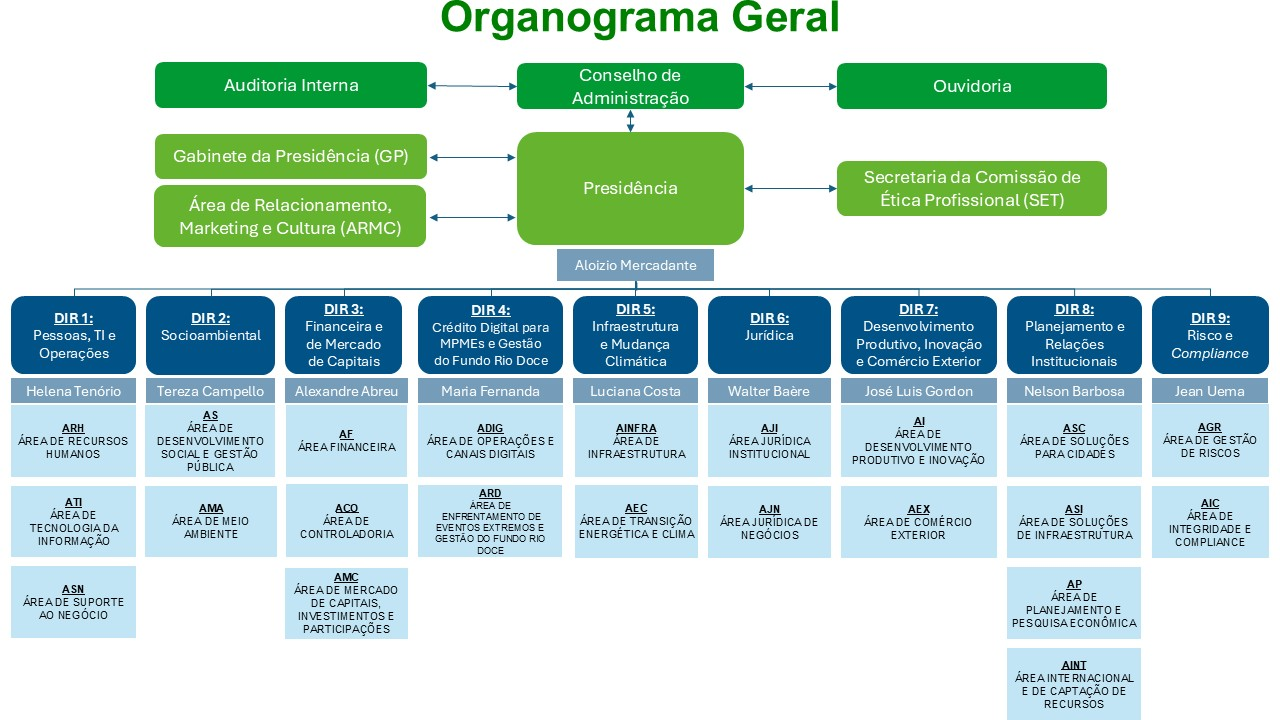
\includegraphics[
        width=\textwidth,
        keepaspectratio
    ]{img/cap_7/organograma_bndes}

    \caption{Organograma do BNDES.}
    \label{fig:organograma-bndes}

    \vspace{0.2cm}
    % \raggedright
    \footnotesize
    Fonte: BNDES (2026).
\end{figure}

% \section{Análise Descritiva da Estrutura organizacional}
% \subsection{Linhas de comunicação -- Formatos e modelos de comunicação interna}

% As linhas de comunicação representam os canais pelos quais informações, decisões, orientações, demandas e resultados circulam entre os diferentes níveis e unidades do BNDES.

% No modelo apresentado pelo documento, observa-se a existência de comunicação vertical \cite[p.~10]{bndes2026oib}, associada às relações de autoridade e subordinação, e de comunicação horizontal ou transversal, decorrente da necessidade de integração entre diferentes Unidades Fundamentais \cite[p.~11]{bndes2026oib}.

% A própria estrutura normativa estabelece que as unidades devem observar as políticas corporativas instituídas pelo Conselho de Administração e as normas operacionais aprovadas pela Diretoria Executiva. Também determina que as unidades planejem, organizem, coordenem e executem suas atividades de acordo com a autoridade superior à qual estão vinculadas.

% \subsection{Unidades de Trabalho -- Níveis de Autoridade}
% Elaborar


% \subsection{Hierarquia -- Cadeias de Comando e Tomada de Decisão}
% A estrutura de governança presente no órgão organiza-se de a partir de linhas claras de autoridade, separação de atribuições e competências deliberativas. Esta informação pode ser encontrada no Estatuto do BNDES \cite{brasil2002estatuto}. Destaca-se:

% \begin{enumerate}
%     \item \textbf{Conselho de Administração} -- constitui o órgão de orientação superior e deliberação estratégica do BNDES, integrando a cúspide da estrutura institucional de governança \cite[p.~24]{brasil2002estatuto}. Composto por conselheiros nomeados pelo Presidente da República e presidido por membro indicado pelo Ministério supervisor, o colegiado tem como núcleo de atuação fixar as diretrizes fundamentais de longo prazo, aprovar o Programa de Dispêndios Globais e apreciar as demonstrações financeiras e os relatórios anuais de auditoria \cite[p.~24]{brasil2002estatuto}. Compete privativamente a este conselho parametrizar os níveis de alçada decisória da Diretoria Colegiada e do Presidente para a aprovação formal de operações financeiras \cite[p.~24]{brasil2002estatuto}.
%     \item \textbf{Diretoria Colegiada} -- atua como o órgão executivo máximo de administração geral, sendo integrada pelo Presidente, pelo Vice-Presidente e por Diretores nomeados pelo Chefe do Poder Executivo Federal \cite[p.~26]{brasil2002estatuto}. É responsável por converter as diretrizes superiores em diretivas práticas de operação, podendo expedir normas e regulamentos de serviços, aprovar o orçamento gerencial e deliberar sobre o organograma interno e a respectiva distribuição de competências. No âmbito financeiro, é quem delibera conclusivamente acerca de operações de crédito cuja esfera financeira se situe na sua faixa de competência estabelecida pelo Conselho de Administração. O Presidente atua como líder da gestão executiva e representação externa do Banco, exercendo poder de veto sobre deliberações da Diretoria submetendo-as ao Conselho de Administração, além de deferir operações monocráticamente, quando aplicáveis \cite[p.~26--27]{brasil2002estatuto}.
%     \item \textbf{Comitês Internos e Instâncias Intermediárias} -- Destacam-se o Comitê de Crédito e Operações (CCOp) e o Comitê de Padronização de Procedimentos Jurídicos (CPPJ). Compete à Área de Gestão de Riscos (AGR) coordenar o CCOp e subsidiar a habilitação e elegibilidade de clientes e operações \cite[p.~35]{bndes2026oib}. Tais instâncias realizam a verificação cadastral, classificação de risco (rating), avaliação socioambiental e mitigação preventiva antes do trâmite às instâncias monocráticas ou executivas \cite[p.~21]{bndes2026oib}
% \end{enumerate}


% \subsection{Divisão Horizontal -- Identificação do Nível Hierárquico}
% Elaborar

\section{Detalhamento dos Componentes Estruturais}

\subsection{Hierarquia: Cadeias de Comando e Tomada de Decisão}

A cadeia de comando do BNDES está alicerçada em uma rígida segregação de competências deliberativas, normativas e executivas, concebida para assegurar conformidade legal, governança pública e sustentabilidade financeira \cite{bndes2025estatuto, bndes2026oib}:

\begin{enumerate}[label=\textbf{\alph*)}]
    \item \textbf{Conselho de Administração (Instância de Orientação e Deliberação Superior):} Composto por 11 (onze) membros eleitos pela Assembleia Geral \cite[art.~33]{bndes2025estatuto}, o Conselho de Administração é o órgão de deliberação máxima e orientação superior do Banco \cite[arts.~17,~I e 18]{bndes2025estatuto}. Compete privativamente ao colegiado:
          \begin{itemize}
              \item Fixar as diretrizes estratégicas, aprovar políticas institucionais (inclusive de governança, integridade, dividendos e pessoal) e subscrever a Carta Anual de Governança \cite[arts.~11 e 36,~VIII e IX]{bndes2025estatuto};
              \item Definir os níveis de alçada decisória para a Diretoria Executiva aprovar e conceder operações \cite[art.~43,~III]{bndes2025estatuto};
              \item Apreciar e manifestar-se sobre as demonstrações contábeis e a destinação de resultados propostas pela Diretoria Executiva, submetendo-as à deliberação da Assembleia Geral \cite[arts.~16,~I, 51,~II e 69]{bndes2025estatuto};
              \item Eleger e destituir os membros da Diretoria Executiva, bem como aprovar metas de gestão \cite[arts.~36,~VII e 39,~\S~1º]{bndes2025estatuto};
              \item Nomear e destituir o Ouvidor Geral, bem como aprovar a designação e destituição do titular da Auditoria Interna mediante proposta do Presidente do Banco \cite[art.~76]{bndes2025estatuto}, \cite[p.~11, itens II.2 e III.2]{bndes2026oib}.
          \end{itemize}
          Para resguardar sua independência, a \textbf{Auditoria Interna (AT)} vincula-se ao Conselho de Administração e ao Comitê de Auditoria \cite[arts.~52 e 57]{bndes2025estatuto}, \cite[p.~11, item II.2; p.~13]{bndes2026oib}. De igual modo, a \textbf{Ouvidoria} está vinculada diretamente ao CA, possuindo independência formal e mandato estrito de 36 meses para seu titular \cite[arts.~75 e 76]{bndes2025estatuto}, \cite[p.~11, item II.5; p.~27]{bndes2026oib}.

    \item \textbf{Diretoria Executiva (Gestão Executiva Superior e Alçadas de Crédito):} Órgão executivo de administração e representação composto pelo Presidente e por 9 (nove) Diretores Executivos eleitos pelo CA \cite[arts.~38 e 39]{bndes2025estatuto}. Possui competência originária para:
          \begin{itemize}
              \item Aprovar a estrutura organizacional e a respectiva distribuição de competências das áreas, mediante proposta do Presidente do Banco \cite[art.~78]{bndes2025estatuto}, \cite[p.~11, itens II.3 e II.4]{bndes2026oib};
              \item Aprovar as linhas orientadoras da ação do BNDES, as normas de operações e as normas de administração mediante regulamentos específicos \cite[art.~43,~II]{bndes2025estatuto};
              \item Deliberar colegiadamente sobre operações financeiras e limites operacionais, observados os limites de alçada estabelecidos pelo Conselho de Administração, sendo permitida a delegação para instâncias executivas no âmbito dos parâmetros normativos internos \cite[art.~43,~III e Parágrafo Único,~I]{bndes2025estatuto};
              \item Fixar limites operacionais e percentuais máximos de participação financeira para programas ou projetos específicos \cite[art.~7º,~Parágrafo Único]{bndes2025estatuto}.
          \end{itemize}
          As deliberações da Diretoria Executiva exigem registro formal em ata com justificativa de dissidências, cabendo ao Presidente a coordenação dos trabalhos, a representação institucional e a faculdade legal de veto submetido ao Conselho de Administração \cite[arts.~40 e 42]{bndes2025estatuto}.

    \item \textbf{Comitês Estatutários de Assessoramento e Comitês Internos:} O arcabouço decisório é apoiado por comitês estatutários obrigatórios previstos na Lei nº 13.303/2016 e pelo Estatuto Social:
          \begin{itemize}
              \item \emph{Comitê de Auditoria:} Vinculado ao CA, atua no monitoramento da integridade contábil, dos controles internos, da Ouvidoria e da Auditoria Interna \cite[arts.~52, 53 e 57]{bndes2025estatuto};
              \item \emph{Comitê de Riscos:} Avalia os limites regulatórios, o apetite institucional e a solvência das operações \cite[arts.~17,~VI e 61]{bndes2025estatuto};
              \item \emph{Comitê de Pessoas, Elegibilidade, Sucessão e Remuneração:} Valida requisitos cadastrais e legais de dirigentes e conselheiros \cite[arts.~21, 59 e 60]{bndes2025estatuto};
              \item \emph{Comitês Operacionais de Apoio:} Colegiados técnicos como o Comitê de Crédito e Operações (CCOp) e o Comitê de Padronização de Procedimentos Jurídicos (CPPJ), atuando na triagem e precificação prévia \cite[p.~21, 35, 163, 172]{bndes2026oib}.
          \end{itemize}

    \item \textbf{Rito de Tramitação Vertical de Financiamentos:} A deliberação sobre apoio financeiro segue um fluxo ascendente mandatório:
          \begin{enumerate}[label=\arabic*.]
              \item \emph{Ingresso e Triagem de Conformidade:} Habilitação cadastral, integridade de contraparte e conformidade regulatória conduzidas pela Área de Integridade e Compliance (AIC) \cite[arts.~7º,~III e 74,~IX e XI]{bndes2025estatuto}, \cite[p.~21, alínea ``q'']{bndes2026oib};
              \item \emph{Instrução Técnica Multidisciplinar:} Análise de viabilidade técnico-econômica, capacidade de pagamento e avaliação de implicações sociais e ambientais realizada pelos Departamentos e Gerências das Áreas operacionais \cite[art.~7º,~I]{bndes2025estatuto}, \cite[p.~45, 63]{bndes2026oib};
              \item \emph{Avaliação de Riscos e Chancelas Jurídicas:} Mensuração do risco de crédito de contraparte pela Área de Gestão de Riscos (AGR) \cite[art.~74]{bndes2025estatuto}, \cite[p.~35, 138]{bndes2026oib} e exame jurídico minucioso pela Área Jurídica de Negócios (AJN) \cite[p.~171--172]{bndes2026oib};
              \item \emph{Deliberação das Alçadas Competentes:} Apreciação pelos comitês intermediários e decisão no âmbito dos limites de alçada delegados ou homologação privativa pela Diretoria Executiva \cite[art.~43,~III e Parágrafo Único,~I]{bndes2025estatuto}.
          \end{enumerate}
\end{enumerate}

\subsection{Unidades de Trabalho: Níveis de Autoridade}

A arquitetura interna do BNDES é dividida em níveis hierárquicos e unidades de trabalho claramente escalonadas no Estatuto e no Caderno OIB \cite[art.~78]{bndes2025estatuto}, \cite[p.~11, item II.4]{bndes2026oib}:

\begin{itemize}
    \item \textbf{Superintendentes de Área (Unidades Fundamentais -- UFs):} Representam o escalão tático-estratégico que lidera as grandes áreas temáticas institucionais \cite[p.~10, item II.1]{bndes2026oib}. Respondem diretamente ao Presidente ou aos Diretores Executivos por delegação deste \cite[arts.~40 e 78]{bndes2025estatuto}, \cite[p.~11, item II.3]{bndes2026oib}. Sua designação e exoneração competem privativamente ao Presidente do Banco \cite[p.~11, item III.3]{bndes2026oib} -- ressalvado o titular da Auditoria Interna, cuja investidura é aprovada pelo Conselho de Administração \cite[p.~11, item III.2]{bndes2026oib}. O Superintendente detém autoridade para planejar, supervisionar orçamentos setoriais, despachar minutas executivas com a Diretoria Executiva e aprovar pareceres técnicos e jurídicos vinculantes no âmbito de sua competência \cite[p.~11, 45, 158, 172]{bndes2026oib}.

    \item \textbf{Chefes de Departamento (Unidades Administrativas Principais -- UAPs):} Constituem o escalão de gestão setorial especializada \cite[p.~11, item II.4]{bndes2026oib}. Exercem autoridade gerencial direta sobre carteiras temáticas. Têm autonomia delegada para coordenar a elaboração de notas e pareceres técnicos, subsídios a políticas públicas, gestão de riscos operacionais inerentes aos seus processos e instrução dos pleitos a serem submetidos às instâncias deliberativas \cite[p.~45, 63, 120, 147]{bndes2026oib}.

    \item \textbf{Gerentes Executivos e Gerentes Setoriais:} Nível de coordenação operacional e supervisão imediata das equipes técnicas de projeto \cite[p.~11, item II.4]{bndes2026oib}. \textbf{Princípio de Segregação Mandatória:} O Estatuto e o Caderno OIB prescrevem como diretriz estruturante que as Áreas e Departamentos Operacionais devem obrigatoriamente designar pelo menos uma gerência especializada exclusivamente no \emph{acompanhamento pós-contratação das operações}, segregando-a funcionalmente das gerências focadas na \emph{análise prévia e concessão de crédito} \cite[art.~74,~XI]{bndes2025estatuto}, \cite[p.~11, item II.7; p.~126]{bndes2026oib}. Essa segregação neutraliza potenciais conflitos de interesse na verificação das condições de eficácia e desembolso.

    \item \textbf{Equipes Técnicas Multidisciplinares (Corpo Técnico Funcional):} Compostas por empregados públicos admitidos mediante concurso público (CLT) \cite[art.~79]{bndes2025estatuto}, abrangendo economistas, contadores, engenheiros, advogados e administradores \cite[p.~11, item II.7; p.~45, 172]{bndes2026oib}. Possuem autonomia funcional para fundamentar notas técnicas, desenhar matrizes de mitigação de risco e atestar a aderência de engenharia e conformidade regulatória \cite[art.~7º,~I]{bndes2025estatuto}, \cite[p.~45, 172]{bndes2026oib}.
\end{itemize}

\subsection{Divisão Horizontal: Identificação do Nível Hierárquico e Especialização}

A distribuição horizontal do BNDES estrutura-se no nível das Unidades Fundamentais (UFs), situadas no mesmo patamar hierárquico sob a supervisão das Diretorias Executivas, aplicando os princípios de especialização técnica, complementaridade e controle mútuo \cite[art.~78]{bndes2025estatuto}, \cite[p.~10--11]{bndes2026oib}:

\begin{enumerate}[label=\textbf{\arabic*.}]
    \item \textbf{Diretorias e Áreas Finalísticas (Fomento e Concessão):} Especializam-se no atendimento setorial às prioridades da política de desenvolvimento e prestação de serviços econômico-financeiros de interesse público \cite[arts.~6º e 7º]{bndes2025estatuto}:
          \begin{itemize}
              \item \emph{Área de Desenvolvimento Produtivo e Inovação (AI):} Apoio ao complexo industrial, inovação e transição tecnológica \cite[p.~43, 45]{bndes2026oib};
              \item \emph{Área de Operações e Canais Digitais (ADIG):} Financiamento descentralizado e automático via rede credenciada de agentes financeiros e garantias de crédito \cite[p.~54, 63, 70]{bndes2026oib};
              \item \emph{Área de Soluções para Cidades, Gestão Pública e Social (ASC/AS):} Estruturação de parcerias de desestatização, infraestrutura urbana, saneamento e inclusão produtiva \cite[art.~6º,~XII e XIII]{bndes2025estatuto}, \cite[p.~87, 118, 120]{bndes2026oib};
              \item \emph{Área de Mercado de Capitais, Investimentos e Participações (AMC):} Subscrição de títulos mobiliários, renda variável e fundos de investimento \cite[art.~43,~III, ``f'']{bndes2025estatuto}, \cite[p.~99--106]{bndes2026oib};
              \item \emph{Área de Comércio Exterior e Área Internacional e de Captação (AINT):} Apoio à exportação e captação de recursos junto a organismos multilaterais \cite[p.~10, 107--113]{bndes2026oib};
              \item \emph{Área de Transição Energética e Climática (AEC):} Fomento à descarbonização, energias renováveis e projetos de combate à mudança climática \cite[art.~6º,~X, ``b'']{bndes2025estatuto}, \cite[p.~111--112]{bndes2026oib}.
          \end{itemize}

    \item \textbf{Diretorias e Áreas Instrumentais, de Controle e Suporte (Gestão Institucional):}
          \begin{itemize}
              \item \emph{Área de Gestão de Riscos (AGR):} Mensuração e controle prudencial dos riscos de crédito, mercado, liquidez, modelo e risco operacional corporativo \cite[art.~74]{bndes2025estatuto}, \cite[p.~35, 138]{bndes2026oib};
              \item \emph{Área de Integridade e Compliance (AIC) e Corregedoria:} Promoção de conformidade, programas anticorrupção, verificação de \emph{background check} e gestão de integridade institucional com independência funcional \cite[arts.~73,~\S~3º e 74]{bndes2025estatuto}, \cite[p.~11, item II.8; p.~21, 29, 33]{bndes2026oib};
              \item \emph{Área de Controladoria (ACO):} Demonstrações financeiras, registros contábeis societários e aderência às regras do CMN \cite[art.~80]{bndes2025estatuto}, \cite[p.~35, 38]{bndes2026oib};
              \item \emph{Áreas Jurídicas Segregadas:} O BNDES adota especialização técnica entre a \textbf{Área Jurídica Institucional (AJI)}, encarregada de governança societária, órgãos colegiados e contencioso judicial \cite[p.~148, 163]{bndes2026oib}, e a \textbf{Área Jurídica de Negócios (AJN)}, focada na estruturação de contratos de financiamento, garantias e captação externa \cite[p.~171--172]{bndes2026oib};
              \item \emph{Área de Recursos Humanos (ARH)}, \emph{Tecnologia da Informação (ATI)} e \emph{Suporte ao Negócio (ASN)}: Gestão de pessoas, suporte logístico e sustentação tecnológica \cite[p.~11, 73, 133, 147]{bndes2026oib}.
          \end{itemize}

    \item \textbf{Interdependência no Modelo das Linhas de Defesa:} A cooperação entre as unidades opera de forma cruzada segundo as diretrizes estatutárias e de governança pública:
          \begin{itemize}
              \item \emph{1ª Linha de Defesa (Unidades Finalísticas Operacionais):} Gerenciam os riscos operacionais e creditícios na sua gênese durante o enquadramento, estruturação e acompanhamento físico-financeiro \cite[art.~7º,~I]{bndes2025estatuto}, \cite[p.~45, 63]{bndes2026oib};
              \item \emph{2ª Linha de Defesa (AGR, AIC, ACO e Áreas Jurídicas):} Estabelecem metodologias, monitoram limites, asseguram a conformidade normativa e fiscalizam o princípio de segregação de funções com independência assegurada \cite[arts.~73,~\S~3º e 74]{bndes2025estatuto}, \cite[p.~21, 33, 35, 172]{bndes2026oib};
              \item \emph{3ª Linha de Defesa (Auditoria Interna -- AT):} Avalia de maneira objetiva e independente a integridade das 1ª e 2ª linhas, subordinada hierarquicamente ao Conselho de Administração \cite[arts.~52 e 57]{bndes2025estatuto}, \cite[p.~11, item II.2; p.~13]{bndes2026oib}.
          \end{itemize}
\end{enumerate}

\subsection{Linhas de Comunicação: Formatos e Modelos de Comunicação Interna}

A formalização da comunicação no BNDES é estritamente regulamentada para assegurar conformidade com as normas da administração pública e mitigar riscos institucionais \cite{bndes2025estatuto, bndes2026oib}:

\begin{itemize}
    \item \textbf{Comunicação Descendente (Fluxo Top-Down -- Normatização e Comando):}
          \begin{itemize}
              \item \emph{Resoluções da Diretoria Executiva:} Instrumentos deliberativos normativos que aprovam políticas corporativas, quadros funcionais, orçamentos e regulamentos específicos de operação \cite[arts.~43,~II e 78]{bndes2025estatuto}, \cite[p.~11]{bndes2026oib};
              \item \emph{Circulares e Ordens de Serviço:} Atos emitidos para uniformizar procedimentos entre departamentos e orientar os agentes financeiros credenciados \cite[p.~44, 172]{bndes2026oib};
              \item \emph{Canais Corporativos e Comunicação Oficial:} Centralizados e orientados institucionalmente conforme detalhado na estrutura da OIB \cite[p.~14, 19]{bndes2026oib}.
          \end{itemize}

    \item \textbf{Comunicação Ascendente (Fluxo Bottom-Up -- Instrução e Reporte Técnico):}
          \begin{itemize}
              \item \emph{Notas Técnicas e Pareceres Multidisciplinares:} Documentos de análise técnica, financeira e socioambiental confeccionados pelas gerências setoriais para instruir as instâncias superiores \cite[art.~7º,~I]{bndes2025estatuto}, \cite[p.~45, 63]{bndes2026oib};
              \item \emph{Manifestações Prévias de Risco e Jurídicas:} Relatórios formais e vinculantes emitidos pela AGR e AJN antes de deliberações de crédito \cite[art.~74]{bndes2025estatuto}, \cite[p.~35, 171--173]{bndes2026oib};
              \item \emph{Relatórios Periódicos de Ouvidoria e Auditoria:} Reportes formais enviados de ofício ao Conselho de Administração e ao Comitê de Auditoria para fins de supervisão \cite[arts.~57,~XXI e 75]{bndes2025estatuto}, \cite[p.~14, 27]{bndes2026oib}.
          \end{itemize}

    \item \textbf{Comunicação Lateral/Transversal (Cooperação Interáreas e Trabalho Colaborativo):}
          \begin{itemize}
              \item \emph{Mecanismo Mandatório de Trabalho Colaborativo:} O Caderno OIB institui expressamente que as unidades organizacionais do BNDES devem adotar rotinas de trabalho colaborativo de forma sistemática como metodologia prioritária de otimização de equipes, desenvolvendo soluções integradas de crédito e mercado de capitais para buscar melhores resultados e maior efetividade no uso dos recursos públicos \cite[p.~11, item II.9]{bndes2026oib};
              \item \emph{Fóruns Técnicos Integrados:} Instâncias multidisciplinares permanentes que reúnem equipes das áreas operacionais, jurídicas e de risco para solucionar gargalos de estruturação econômico-financeira de grandes projetos \cite[p.~11, item II.9; p.~120, 163]{bndes2026oib}.
          \end{itemize}
\end{itemize}

\subsection{Considerações}

A macroestrutura organizacional e hierárquica do BNDES reflete fielmente as diretrizes de governança corporativa da Lei nº 13.303/2016 e do seu Estatuto Social vigente, equilibrando uma governança colegiada e estratégica nas instâncias superiores com unidades operacionais setoriais especializadas, contrapesadas de forma autônoma pelas áreas de risco, controle, integridade e auditoria interna.


% ================================================================
% ELEMENTOS PÓS-TEXTUAIS
% ================================================================

\bibliographystyle{abntex2-alf}
\bibliography{referencias}

\end{document}
